\section{View}
\label{chap:view_impl}
The view in this project is implemented based on the concept designed in \autoref{chap:view_design}. 
During the implementation of the UI, some adjustments were made to better support the functionalities and enhance the overall appearance of the application.
While the design mockups provided a solid foundation, certain adjustments were necessary to improve the overall user experience.
The adjustments include color themes and font to ensure readability and consistent appearance.

\subsection{MainActivity}
The user interface displays several functionalities to fulfill the requirements of the system described in \autoref{chap:requirements}. To promote separation of concerns, the user interface is implemented in several \texttt{Fragment}, improving the code readability and maintainability.  
\texttt{MainActivity} serves as the container that binds the fragments together. \texttt{FragmentContainerView}\footnote{\url{FragmentContainerView} is a customized Layout designed specifically for Fragments. URL: \url{https://developer.android.com/reference/androidx/fragment/app/FragmentContainerView}} is used to host and display different fragments based on the user's navigation.
The navigation between the fragments is controlled by the Android Navigation\footnote{\url{Navigation} is a framework provided by the Android Jetpack library that simplifies the implementation of navigation in an Android app. URL: \url{https://developer.android.com/guide/navigation}}, which is configured in a XML file. 

The \texttt{MainActivity} provides a bottom navigation tool for users to navigate between the fragments. It is implented using the \texttt{BottomNavigationView}\footnote{\url{BottomNavigationView} represents a standard bottom navigation bar for application. URL: \url{https://developer.android.com/reference/com/google/android/material/bottomnavigation/BottomNavigationView}}.
The bottom navigation tool differs slightly from the original mockup. It displays self-explanatory icons to improve user understanding. The goal of the change is to make navigation more intuitive for the users by using easily understandable icons. The change aims to create a user-friendly interface and improve the user experience. 
\begin{figure}[H]
    \centering
    
\includegraphics[width=0.75\textwidth]{images/bottom-navbar.png}
    \caption{Screenshot of the bottom navbar}
    \label{fig:bottom_navbar}
\end{figure}

Additionally, \texttt{MainActivity} manages permission requests to ensure the necessary permissions are granted for the app's functionality. Specifically, it requests the \texttt{ACCESS\_COARSE\_LOCATION} permission.

\subsection{HomeFragment}
The implementation of \texttt{HomeFragment} includes several feature to fulfill the requirements of the system. 
The implementation follows the concept designed in \autoref{chap:home_design} with some adjustments.
The information regarding the user's current heart rate and current activity is presented within a card layout to enhance the visual appearance and to provide clear and structured display.

\texttt{HomeFragment} provides a switch to control the connection to the heart rate sensor. 
The switch is implemented using MaterialSwitch from MaterialDesign to easily handle the behavior of the switch when toggled on and off to start or stop the connection to the heart rate sensor.
This feature is disabled when there is no active user, preventing unwanted connection to heart rate sensor.

Moreover, the fragment displays the user's current heart rate (bpm) by observing the \texttt{currentHrBpm} LiveData from the \texttt{HrViewModel}. This ensures that the displayed heart rate is always up-to-date.
Additionally, the \texttt{HomeFragment} shows the user's current activity intensity level by observing the \texttt{currentActivity} LiveData also provided by the \texttt{HrViewModel}. 

Furthermore, the fragment features an interactive graph that visualizes the user's heart rate data over time. 
The graph is controlled by another component called \texttt{GraphService} using the MPAndroidChart library, specifically the \texttt{LineChart} class.
The \texttt{GraphService} subscribes to the \texttt{HrEventBus}, which broadcasts heart rate data events. 
Whenever a heart rate data event is received, the \texttt{GraphService} updates the data set associated with the graph. 
This ensures that the graph is continuously updated with the latest heart rate data.
Additionally, the \texttt{GraphService} also reacts to active user change. 
When the active user is changed, the \texttt{GraphService} generates a new graph based on the heart rate data of the new active user. 

Overall, the \texttt{HomeFragment} observes the current active user and dynamically updates the user interface to display the current heart rate, activity level, and the graph.
\begin{figure}[H]
    \centering
    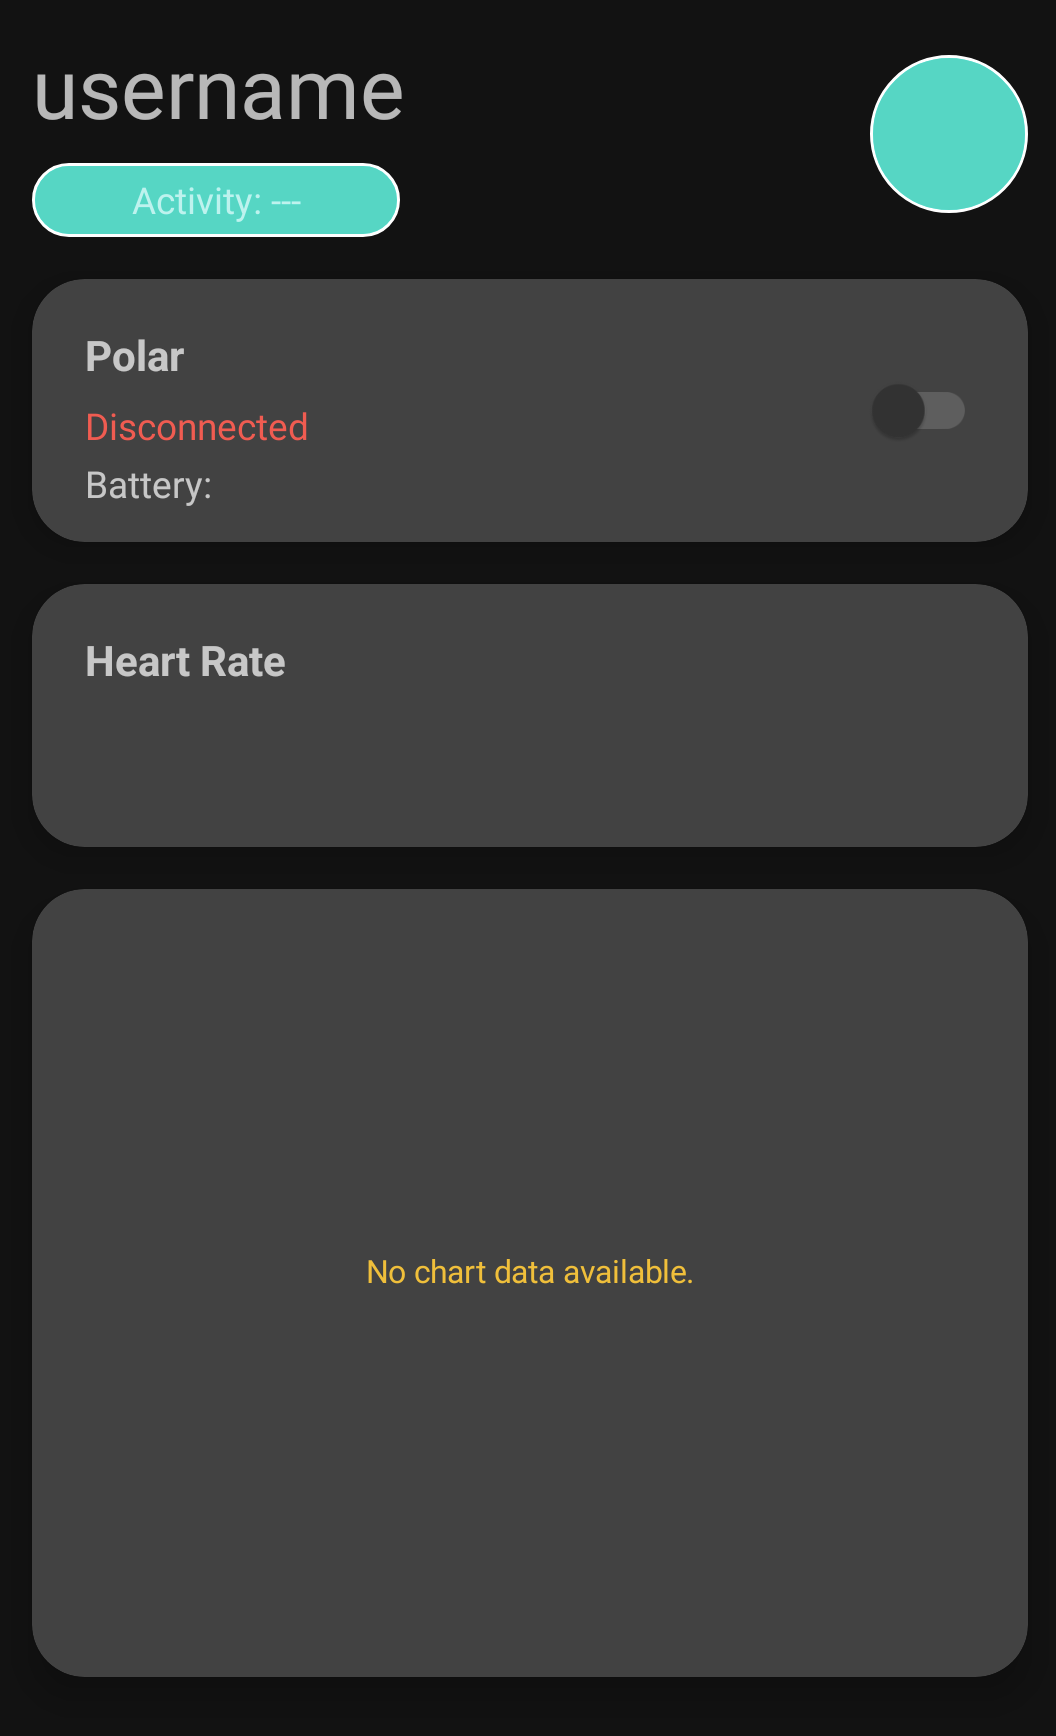
\includegraphics[width=0.5\textwidth]{images/homefragment-screenshot.png}
    \caption{Screenshot of HomeFragment}
    \label{fig:homefragment_screenshot}
\end{figure}

\subsection{ExerciseFragment}
The \texttt{ExerciseFragment} is implemented according to the design in \autoref{chap:exercise_design}, with some adjustments made to improve the user experience.
It provides more details about the ongoing exercise, such as the maximum, minimum, and average heart rate bpm, as well as the start time of the exercise.
The \texttt{ExerciseFragment} shows an overview of an ongoing exercise. It uses \texttt{DataBinding} to display the exercise details and observing the \texttt{currentExercise} LiveData from the \texttt{ExerciseViewModel}. 
The \texttt{ExerciseFragment} also offers buttons to start and stop an exercise session. The buttons are implemented using MaterialButton to allow further color and shape customization.
Once the user presses the button to start an exercise session and the session is successfully started, the start button will be automatically disabled to prevent multiple start requests. Similarly, when the stop button is pressed, the stop button will also be disabled to avoid any unintended interruptions. 
This approach ensures that the exercise can be performed without any conflicting or overlapping commands.
To ensure accurate data, the \texttt{ExerciseFragment} observes the current active user and adjusts the exercise information accordingly.

Additionally, a separate fragment called \texttt{ExerciseListFragment} is created inside the \texttt{ExerciseFragment} to display a history of completed exercises, along with their detailed information, allowing users to track their progress over time. The \texttt{ExerciseFragment} observes \texttt{currentExerciseList} live data from the \texttt{ExerciseViewModel} to receive updates. 
\texttt{RecyclerView}\footnote{\url{RecyclerView} is widget used for displaying sets of data efficiently. URL: \url{https://developer.android.com/reference/androidx/recyclerview/widget/RecyclerView}} widget is used to dynamically display the \texttt{currentExerciseList} in a scrollable view. 
Each completed exercise shown in the \texttt{RecyclerView}, along with its details, is contained within in a card layout.

\begin{figure}[H]
    \centering
    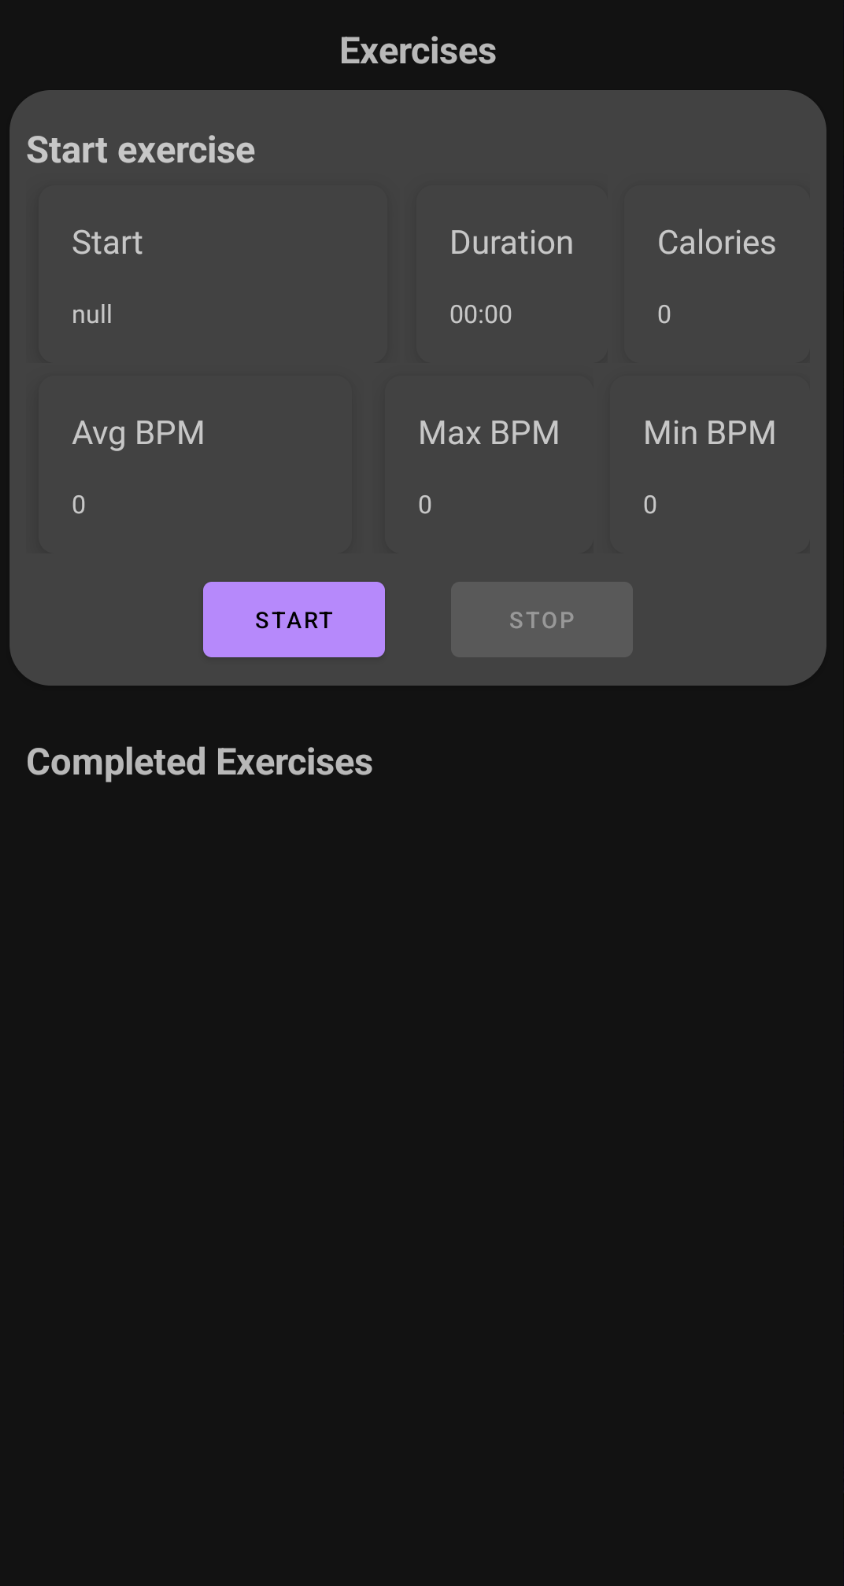
\includegraphics[width=0.5\textwidth]{images/exercisefragment-screenshot.png}
    \caption{Screenshot of ExerciseFragment}
    \label{fig:exercisefragment_screenshot}
\end{figure}

\subsection{UserFragment}
The implementation of the \texttt{UserFragment} follows the concept discussed in \autoref{chap:user_design} with some modifications. 
The \texttt{UserFragment} is responsible for displaying the details of the current active user and providing the user an interface to manage their own data, for instance, update or delete their data. 
To achieve this functionality, it observes the \texttt{currentUser} LiveData from the \texttt{UserViewModel} and bind it using \texttt{DataBinding}. 
The user information is displayed in text fields and a calendar is available to support adding or editing the date of birth. 
Additionally, \texttt{UserFragment} provides three buttons for deleting, adding, and updating user data. Similar to the buttons in the \texttt{ExerciseFragment}, they are also implemented using MaterialButton, allowing further color and shape customization to be more visually appealing.
\begin{figure}[H]
    \centering
    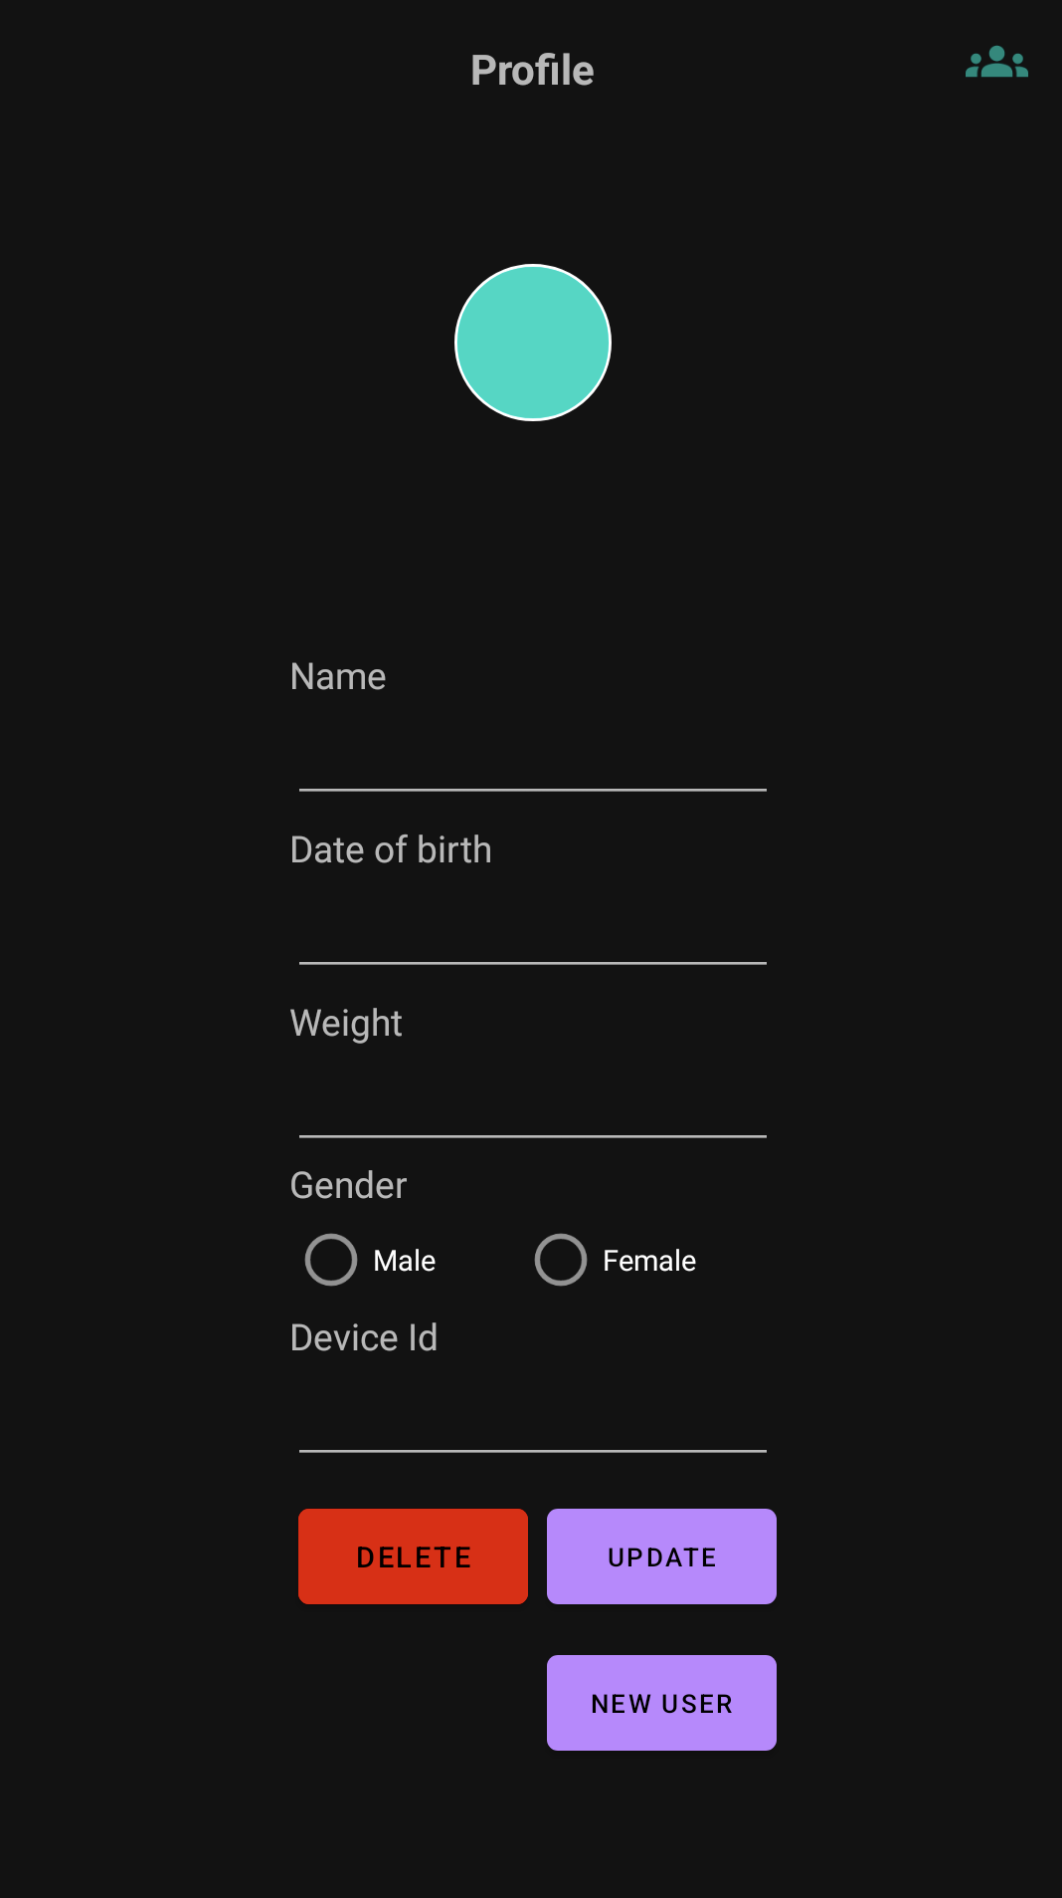
\includegraphics[width=0.6\textwidth]{images/userfragment-screenshot.png}
    \caption{Screenshot of UserFragment}
    \label{fig:userfragment_screenshot}
\end{figure}

Furthermore, a separate \texttt{UserListFragment} is implemented to display a list of all users in the system. 
To keep the \texttt{UserListFragment} up-to-date with the latest users in the database, it observes the \texttt{users} LiveData from \texttt{UserViewModel}, which contains the actual list of all users in the database. 
This ensures that the newest user is included in the list as soon as it is inserted. By using LiveData, the \texttt{UserListFragment} remains synchronized with the user data, providing a real-time view of all users.
Similar to the \texttt{ExerciseListFragment}, it uses a \texttt{RecyclerView} to display a list of users. 
Each user in the list is contained within a clickable card, allowing active user change by selecting a different user from the list.
\begin{figure}[H]
    \centering
    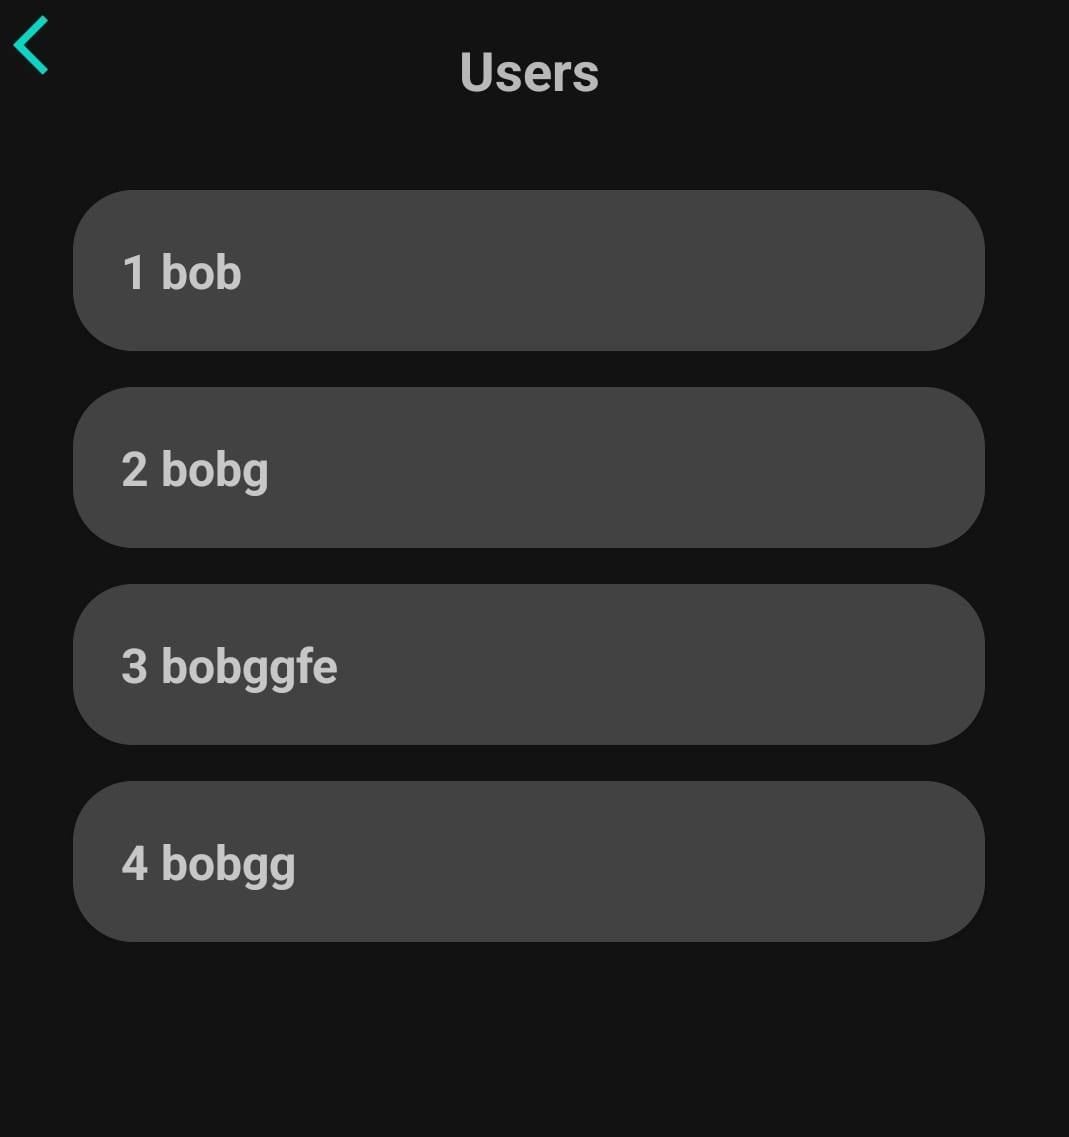
\includegraphics[width=0.6\textwidth]{images/userlistfragment-screenshot.jpeg}
    \caption{Screenshot of UserListFragment, containing list of all users}
    \label{fig:userlistfragment}
\end{figure}


